\begin{figure}[ht]
\centering
	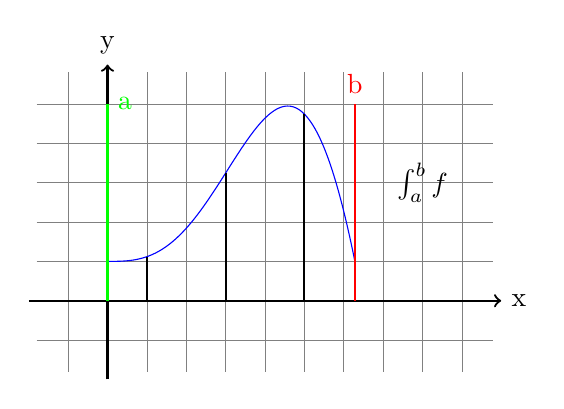
\begin{tikzpicture}
		\draw[very thin, gray, step = 0.5] (-0.9,-0.9) grid (4.9,2.9);
		\draw[->,thick, black](-1,0) -- (5,0) node[right]{x};
		\draw[->,thick, black](0,-1) -- (0,3) node[above]{y};
		\draw[blue,domain = 0.0:3.14, samples=1000]   
			plot (\x,{(\x * \x)*sin(\x r)*0.5+0.5});
       	\draw[green,thick](0.0,0)--(0.0,2.5)node[right]{a};
       	\draw[red,thick](3.14,0) -- (3.14,2.5) node[above]{b};
       	\draw[black,thick](0.5,0) -- (0.5, 0.56);
       	\draw[black,thick](1.5,0) -- (1.5, 1.62);
       	\draw[black,thick](2.5,0) -- (2.5, 2.37);
       	\node at (4,1.5){$\int_a^b f$};
	\end{tikzpicture}
\end{figure}